\pagestyle{plain}  % kvuli cislovani stranek

\chapter{Sada nástrojů, Úvod??}

Relativně nedávno vzniklé NoSQL a další moderní databázové systémy umožnily vytvářet databáze založené na jiných logických modelech než jen na tradičních relačních (např. klíč-hodnota, dokumentové, grafové). I když některé systémy vypadají podobně, neexistují mezi nimi univerzální standardy, které by nám umožnily zaměnitelné použití. Částečné řešení lze nalézt u multi-modelových databází. Do jednoho systému lze začlenit více modelů tak, že spolu koexistují v různých vzájemně propojených formátech a modelech. Propojení může fungovat různými způsoby. Jeden model může být vlžen do druhého, entity z jednoho ukazující na entity z druhého, nebo redundance dat uložena ve více modelech. Stále ale neexistuje obecný způsob, jak modelovat multi-modelová data, nebo je transformovat z jednoho modelu do druhého.

Problémem jednotného modelování a reprezentace dat, jako i řízení jejich vývoje, se zabývají P. Koupil a I. Holubová v článku o jednotné reprezentaci a transformaci multi-modelových dat pomocí teorie kategorií (category theory) \cite{cat_theory}. Snaží se formálně podchytit výše zmiňované problémy. Jejich přístup umožňuje propojit různé modely a vybírat způsob kombinace. Další výhodou je jednotné dotazování nad daty, migrace mezi modely a vývoj modelu a sním i dat. Všechno by mělo být možné bez nutnosti znát specifika propojených modelů. Zároveň je docíleno určité jednoduchosti v návrhu díky tomu, že teorii kategorií převádějí na grafovou reprezentaci. Uvádějí, že je pak praktické využití snažší.

V návaznosti na přístup pomocí teorie kategorií vzniklo několik článků, které navrhují, jak implementovat teoreticky navržené funkcionality. Ne všechna data mají předem definované schéma. Funkčnost MM-infer \cite{MM_infer} se snaží schéma zpětně zrekonstruovat z~již uložených multi-modelových dat. Dotazováním nad multi-modelovými daty se zabývá článek o MM-quecat \cite{MM_quecat}. A v neposlední řadě evoluci dat navrhuje článek o MM-evocat \cite{MM_evocat}. Funkcionality a k nim vznikající nástroje, byly většinou vytvářeny odděleně. 

Protože se funkce hodí k využití propojené (nechceme se dotazovat nad multi-modelovými daty bez možnosti jejich vytvoření, vytvořená schémata bychom rádi ještě upravovali apod.), vznikl nástroj MM-cat \cite{MM_cat}, který se je postupně snaží sjednotit.

\section{MM-cat}
MM-cat framework je navržený tak, aby řešil složitosti spojené s~návrhem a~správou multi-modelových databází. Jeho hlavním úkolem je vytvářet kategorický model (multi-modelové schéma). Umí ho dekomponovat a~umožňuje uživateli, aby si zvolil mapování na příšlušné DBMS (Database Management System). Kategorický model, mapování a~základy konceptuálního modelování popisuje článek MM-evocat \cite{MM_evocat}. Řeší i případy, kdy se struktura dat v~čase mění tak, aby například vyhovovala novým uživatelským požadavkům. Takové změny jsou pak propagovány napříč definovanými modely a~datovými instancemi. Slouží i~jako základ pro rozšíření o~složitější úkoly. 

MM-cat je framework, který má zatím nedokončené grafické webové rozhraní. Při vzniku nástroje nebyl kladený důraz na jeho návrh a možnosti dalšího rozšíření. Proto se následující práce zabývá návrhem nového uživatelského rozhraní, které má být vytvořeno nezávisle na existujícím. 

Když se podíváme třeba na otevřené schéma (Obr. \ref{obr01:mm-cat}) ve webové aplikaci, objevují se v pravé i levé dolní liště tlačítka, která často nemají žádnou funkci. Levá lišta se mění na jinou po přístupu do jiných částí aplikace, což alespoň ze začátku používání aplikace může být matoucí.

\begin{figure}[htb]
  \centering
  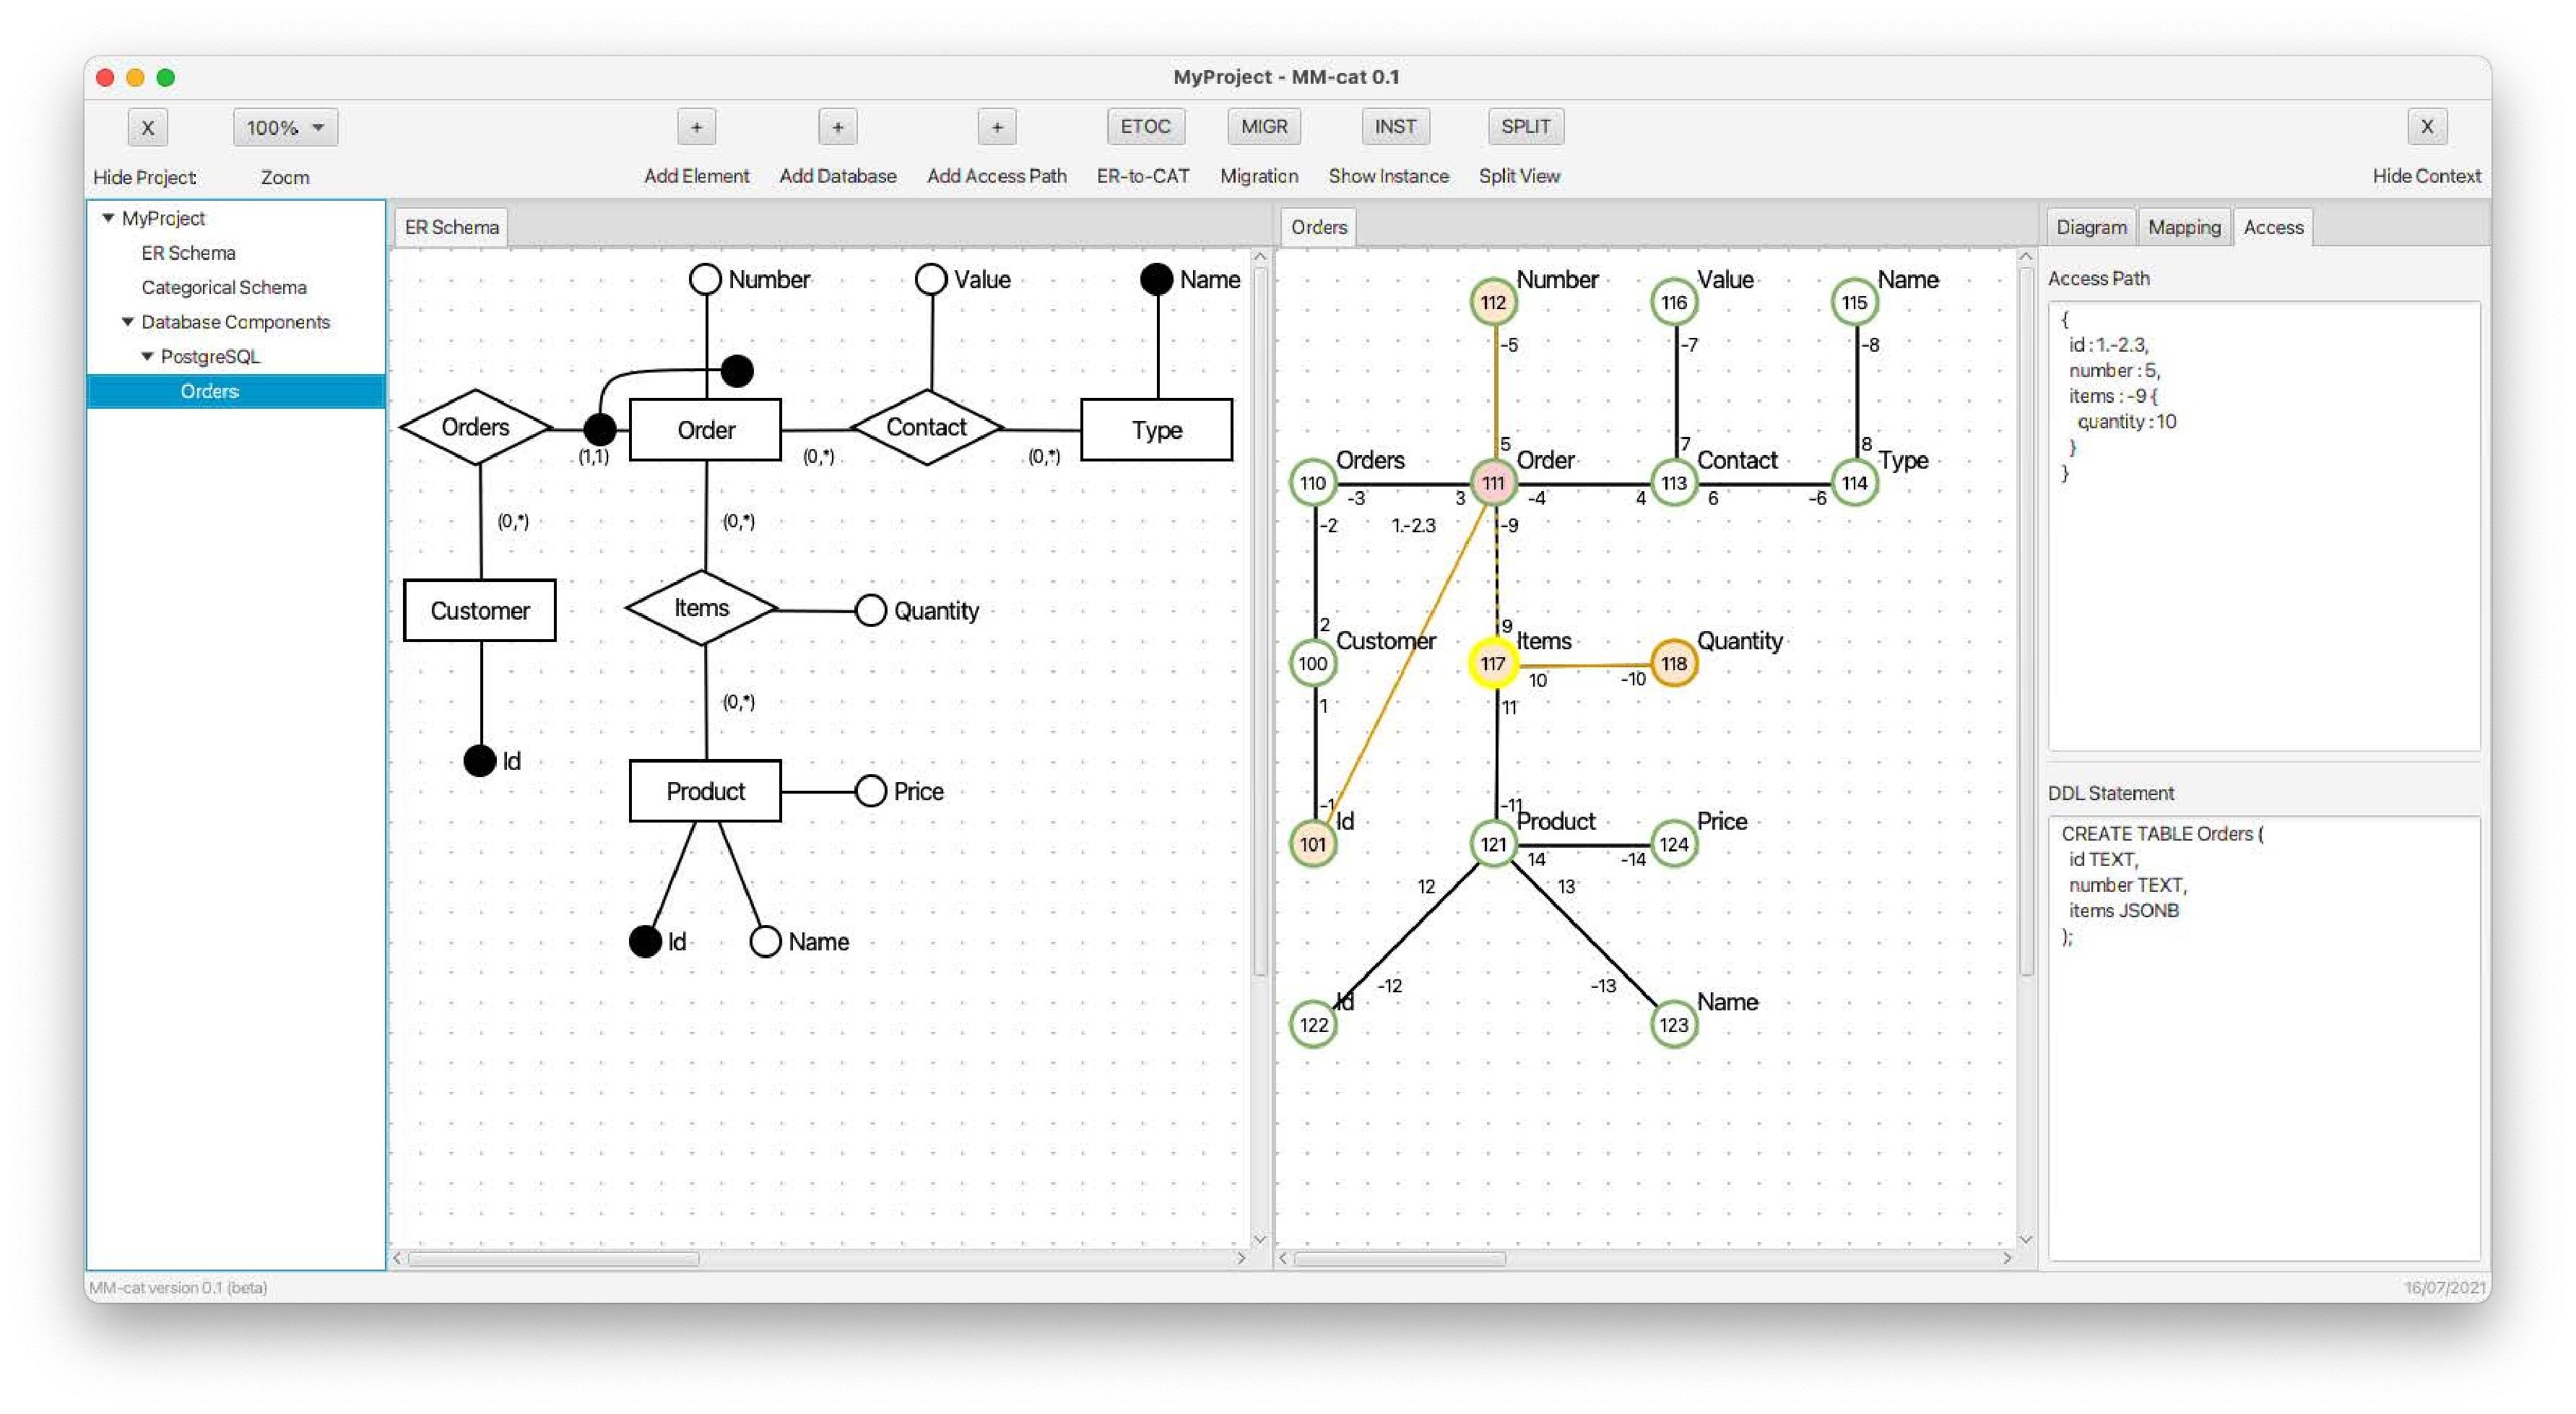
\includegraphics[height=90mm]{../img/mm-cat}
  \caption{Ukázka uživatelského rozhraní nástroje MM-cat.}
  \label{obr01:mm-cat}
\end{figure}

V horní liště je pak umístěný název otevřeného schématu „Basic Schema“. Pozice v liště, která vypadá jako navigační menu, nemusí být intuitivní. Na další omezení a nejasnosti uživatel narazí při dalším používání. Často je potřeba podívat se do dokumentace, co vlastně nástroj dělá a která tlačítka fungují.

\section{Postup návrhu uživatelského rozhraní}

Návrh uživatelského rozhraní jsme rozdělili do 4 bodů. Začneme definováním cílových skupin uživatelů, kteří budou aplikaci používat. O tom proč je důležité začít právě tímhle se zabývají autoři knihy Designing Interfaces \cite{Designing_ifaces_2nd_edition} na začátku první kapitoly.

Následuje definování běžných úkolů, které budou uživatelé v aplikaci dělat, a hierarchická analýza úkolů (HTA). Tím si načrtneme představu o všech krocích, které povedou ke splnění úkolu.

Storyboardy budou další zastávkou. Můžeme si je představit jako komiksy o plnění úkolů uživateli se zdárným koncem. Díky tomu se zamyslíme, jak se uživatelé chovají při plnění úkolů.

Nakonec vytvoříme papírový prototyp aplikace a otestujeme jeho použitelnost na reálných uživatelích.
